\subsection{Audio, PWM}\label{sec:audioPWM}
Um ein Audiosignal abspielen zu können, werden zwei PWM-Signale benötigt wie in Abbildung \ref{fig:pwm_ausgang}. Das einte Signal ist die invertierte Variante des anderen Signals. 
Das PWM-Signal wird mit dem NRF52 generiert. Für den NRF52 stellt NORDIC SEMICONDUCTOR die PWM HAL and driver Bibliothek zu Verführung, die es ermöglicht ein PWM zu erzeugen. Der NRF52 bietet vier PWM Instanzen mit je vier Kanälen. Für die Audioausgabe wurden zwei PWM Instanzen mit je einem Kanal genutzt. Im folgenden Abschnitt wird erklärt wie ein PWM Signal eines Kanales generiert wurde.

\begin{figure}[H]
	\begin{center}
		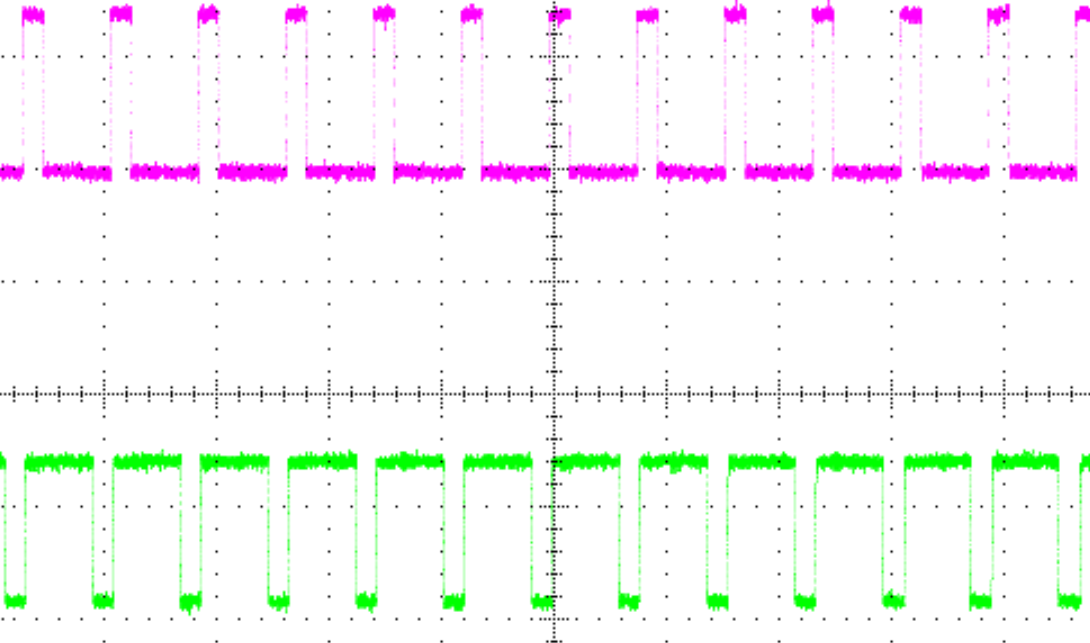
\includegraphics[width=80mm]{data/PWM_Signal_500Hz_Mono}
		\caption[PWM-Ausgang des NRF52]{PWM-Ausgang des NRF52. Das violette Signal ist das invertiere grüne Signal.} %picture caption
		\label{fig:pwm_ausgang}
	\end{center}
\end{figure}

In der Abbildung \ref{fig:pwm_ablauf} ist der Ablauf des PWM-Unterprogramm aufgezeigt. Als erstes findet die Initialisierung statt. Nach der Initialisierung können die beiden Sequenzen 0 und 1 generiert werden. In diesen Sequenzen sind die wav file Daten abgelegt. Die Funktion complex\_playback generiert am Ausgang anhand diesen Sequenzen ein PWM Signal.

\begin{figure}[H]
	\begin{center}
		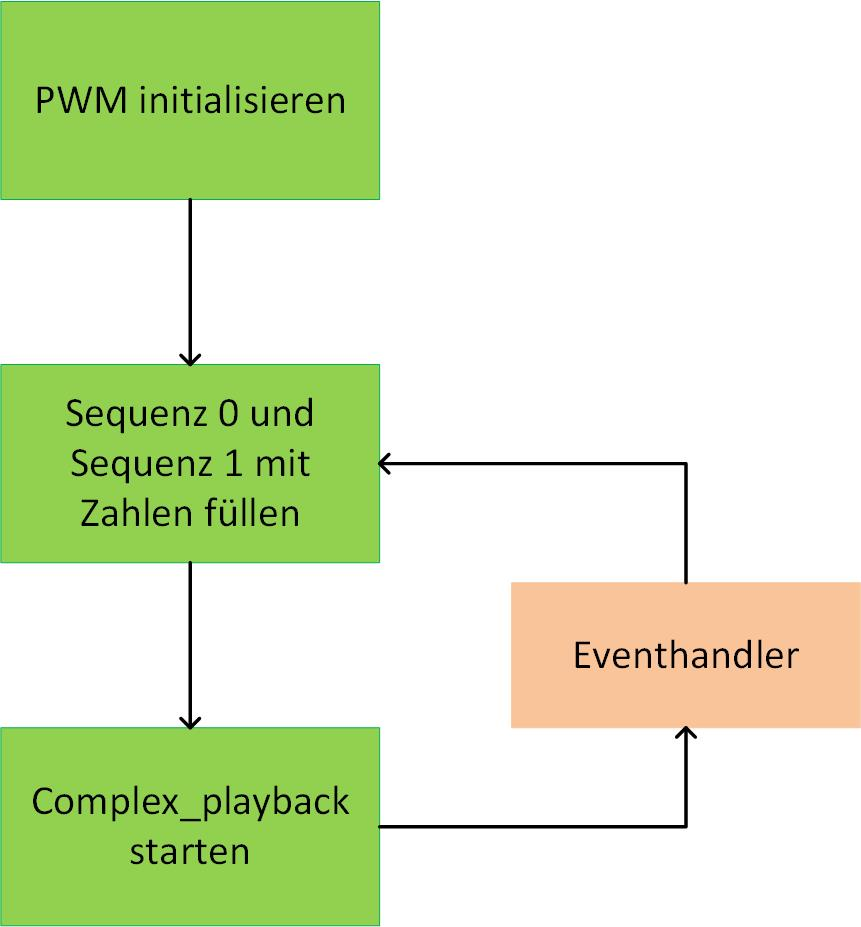
\includegraphics[width=80mm]{data/pwm_ablauf.jpg}
		\caption[Ablauf PWM]{Ablauf PWM} %picture caption
		\label{fig:pwm_ablauf}
	\end{center}
\end{figure}

\subsubsection*{PWM Initialisieren}\label{sec:PWM initialisieren}
Definieren der Abtastfrequenz
-Welche PWM Instanz\\
-Config\\
	*ouputPins\\
	*clock\\
	*zählermodus\\
	*top value\\
	*Kanal modus\\
	*modus\\
-event handler

Da die clock Frequenz des PWM Moduls auf $16MHz$ gesetzt wurde, beträgt der top value für eine Audiodatei mit Abtastfrequenz von $32kHz 500$. Dies berechnet sich wie folgt:
\begin{equation}
32kHz = \frac{16MHz}{top value}
top value = \frac{16MHz}{32kHz} = 500
\end{equation}

\subsubsection*{Sequenzen befüllen}\label{sec:Sequenzen befüllen}
Daten in sequenzen füllen, seqeuenz 1 muss noch ein Datenwert dazugerechnet werden. verweisen auf die SD Kart lesefunktion.

\subsubsection*{Complex playback}\label{sec:Complex playback}
Die Funktion generiert anhand der Sequenz eine PWM-Signal. Der
Vorteil zu simple playback ist das zwei sequenzen mitgegeben werden können. Wenn die Sequenz 0 fertig abgespielt wurde, startet automatisch die zweite Sequenz und der eventhandler wird ausgelöst. In dieser Zeit kann die erste Sequenz wieder neu beladen werden. Die Beladung der Sequenzen wird mit dem eventhandler dieser Funktion gesteuert. 

\begin{table}[H]
	\centering
	\begin{tabular}{|l|l|l|}
		\hline
		%\rowcolor[HTML]{C0C0C0} 
		\textbf{Beschreibung} & \textbf{Funktion}                & \textbf{Argumente}                                                                                                                                                                                                            \\ \hline
		PWM initialisiern     & nrf\_drv\_pwm\_init              & \begin{tabular}[c]{@{}l@{}}nrf\_drv\_pwm\_t const *const p\_instance\\ nrf\_drv\_pwm\_config\_tconst *p\_config\\ nrf\_drv\_pwm\_handler\_thandler\end{tabular}                                                               \\ \hline
		Audio abspielen         & nrf\_drv\_pwm\_complex\_playback & \begin{tabular}[c]{@{}l@{}}nrf\_drv\_pwm\_t const *const p\_instance\\ nrf\_pwm\_sequence\_t const *p\_sequence\_0\\ nrf\_pwm\_sequence\_tconst *p\_sequence\_1\\ uint16\_t  playback\_count \\ uint32\_t  flags\end{tabular} \\ \hline
	\end{tabular}
	\label{my-label}
	\caption{Funktionen der PWM HAL and driver Bibliothek}
\end{table}
